\documentclass[letter,11pt]{article}
\usepackage{latexsym}
\usepackage{xcolor}
\usepackage{float}
\usepackage{amsthm}
\usepackage{amssymb}
\usepackage{wrapfig}
\usepackage{tabularx}
\usepackage{titlesec}
\usepackage{subcaption}
\usepackage{tikz}
\usepackage{import}
\usepackage{geometry}
\usepackage{verbatim}
\usepackage{enumitem}
\usepackage{standalone}
\usepackage{fancyhdr}
\usepackage{pgfornament}
\usepackage{multicol}
\usepackage{pgfplots}
\usepackage{graphicx}
%\usepackage{cfr-lm}
\usepackage{booktabs}
\usepackage{svg}
\usepackage[T1]{fontenc}
\pgfplotsset{compat=1.17}
\setlength{\multicolsep}{0pt}
\pagestyle{fancy}
%\fancyhf{} % clear all header and footer fields
\fancyhead{}\fancyfoot{}
\fancyhead[R]{\textbf{\thepage}}
\fancyhead[L]{Aiden M. Rosenberg, MMXXIII A.D. }
\addtolength{\headwidth}{3cm}


\renewcommand{\headrulewidth}{1pt}
\renewcommand{\footrulewidth}{0pt}
\geometry{left=1.5cm, top=2.5cm, right=1.5cm, bottom=2cm}

%\usepackage{draftwatermark}
%\SetWatermarkColor[gray]{0.9}
%\SetWatermarkText{Private}
%\SetWatermarkScale{3}

\usepackage[most]{tcolorbox}
\tcbset{
	frame code={}
	center title,
	left=0pt,
	right=0pt,
	top=0pt,
	bottom=0pt,
	colback=gray!20,
	colframe=white,
	width=\dimexpr\textwidth\relax,
	enlarge left by=-2mm,
	boxsep=4pt,
	arc=0pt,outer arc=0pt,
}


\raggedright
\setlength{\tabcolsep}{0in}

% Sections formatting
\titleformat{\section}{
  \vspace{-4pt}\scshape\raggedright\large
}{}{0em}{}[\color{black}\titlerule \vspace{-7pt}]

\pgfplotsset{compat=1.17}

\begin{document}
\thispagestyle{empty}

\fontfamily{cmr}\selectfont
%----------HEADING-----------------

\parbox{2.35cm}{%
	\includegraphics[width=2.3cm]{logo.png}
}
\parbox{0.3cm}{\hspace{0.3cm}}
\parbox{\dimexpr\linewidth-5cm\relax}{
	\setlength{\tabcolsep}{0.5em}
	\def\arraystretch{1.25}
	\begin{tabular}{@{}llll@{}}
		\toprule
		\multicolumn{4}{c}
		{\hspace{-0.5em}\textbf{Assignment}: Worksheet \# 2 (13.6, 15.1)} \\ \midrule
		\textbf{Name:}   & D. Aiden M. Rosenberg & \textbf{Professor:} & Dr. Alan v. Herrmann Ph.D \\
		\textbf{Course:} & Calculus III          & \textbf{Date:}      & August 24th, 2023 A.D.    \\ \bottomrule
	\end{tabular}
}
\vspace{1cm}

\section{Cylinders and Quadratic Surfaces}
\subsubsection{}
Consider the following surface $$z=16-\frac{x^2}{4}-y^2$$
\begin{enumerate}[label=\Alph*.]
	\item Find $x-$, $y-$, and $z-$intercepts if they exist.
	      \begin{enumerate}
	      	\item $\underbrace{x-\text{intercept}}_{(y=0 \text{ and } z=0)}:  0 = 16-\frac{x^2}{4} \Longrightarrow x= \pm 8$
	      	\item $\underbrace{y-\text{intercept}}_{(x=0 \text{ and } z=0)}:  0 = 16-y^2 \Longrightarrow y= \pm 4$
	      	\item $\underbrace{z-\text{intercept}}_{(x=0 \text{ and } y=0)}:  0 = 16-y^2 \Longrightarrow z= 16$
	      \end{enumerate}
	\item Determine equations for the traces in the $xy-$, $yz-$, and $xz-$planes, if they exist, and graph these traces in the coordinate planes.
	      	      
	      \begin{figure}[h]
	      	\centering
	      	\begin{subfigure}{0.3\textwidth}
	      		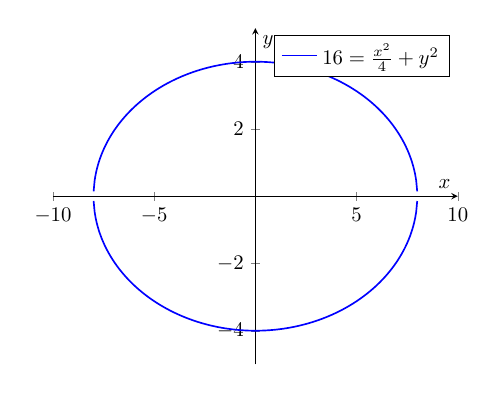
\begin{tikzpicture}[scale=0.75]
	      			\begin{axis}[
	      					xlabel=$x$,
	      					ylabel=$y$,
	      					axis lines=middle,
	      					xmin=-10, xmax=10,
	      					ymin=-5, ymax=5,
	      					samples=400, % Increase for smoother curve
	      					domain=-10:10,
	      				]
	      				\addplot+[color=blue,mark=none,thick,restrict y to domain=-10:10] {sqrt(16-x^2/4)};
	      				\addplot+[color=blue,mark=none,thick,restrict y to domain=-10:10] {-sqrt(16-x^2/4)};
	      				\addlegendentry{$16=\frac{x^2}{4}+y^2$}
	      			\end{axis}
	      		\end{tikzpicture}
	      		\caption{$xy-$trace}
	      	\end{subfigure}
	      	\begin{subfigure}{0.3\textwidth}
	      		\begin{tikzpicture}[scale=0.75]
	      			\begin{axis}[
	      					xlabel=$y$,
	      					ylabel=$z$,
	      					axis lines=middle,
	      					xmin=-10, xmax=10,
	      					ymin=0, ymax=20,
	      					samples=400, % Increase for smoother curve
	      					domain=-10:10,
	      				]
	      				\addplot+[color=red,mark=none,thick,restrict y to domain=-20:20] {16-x^2};
	      				\addlegendentry{$z=16-y^2$}
	      			\end{axis}
	      		\end{tikzpicture}
	      		\caption{$yz-$trace}
	      	\end{subfigure}
	      	\begin{subfigure}{0.3\textwidth}
	      		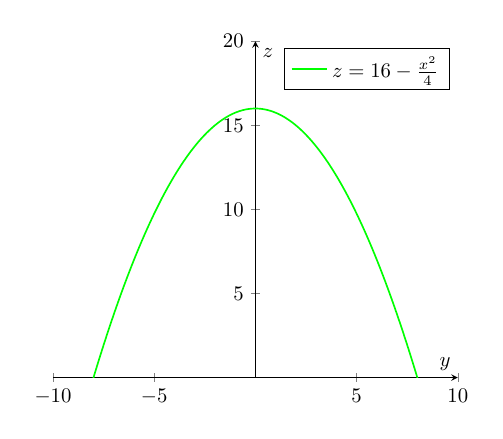
\begin{tikzpicture}[scale=0.75]
	      			\begin{axis}[
	      					xlabel=$y$,
	      					ylabel=$z$,
	      					axis lines=middle,
	      					xmin=-10, xmax=10,
	      					ymin=0, ymax=20,
	      					samples=400, % Increase for smoother curve
	      					domain=-10:10,
	      				]
	      				\addplot+[color=green,mark=none,thick,restrict y to domain=-20:20] {16-(x^2)/4};
	      				\addlegendentry{$z=16-\frac{x^2}{4}$}
	      			\end{axis}
	      		\end{tikzpicture}
	      		\caption{$yz-$trace}
	      	\end{subfigure}
	      \end{figure}
	      	      
	\item Graph the surface.
	      \begin{figure}[h]
	      	\centering
	      	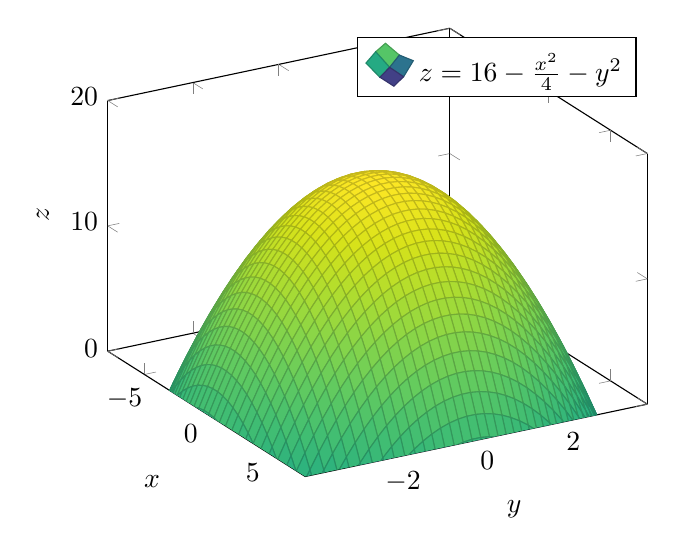
\begin{tikzpicture}
	      		\begin{axis}[
	      				xlabel=$x$,
	      				ylabel=$y$,
	      				zlabel=$z$,
	      				domain=-10:10,
	      				y domain=-5:5,
	      				zmin=0,
	      				zmax=20,
	      				samples=50,
	      				colormap/viridis,
	      				view={60}{30},
	      			]
	      			\addplot3[surf] {16 - x^2/4 - y^2};
	      			\addlegendentry{\(z=16-\frac{x^2}{4}-y^2\)}
	      		\end{axis}
	      	\end{tikzpicture}
	      	\caption{Parabolic Ellipsoid}
	      \end{figure}
\end{enumerate}
\newpage
\subsubsection{}
Traces are provided for each of the following surfaces on the next page. Match the traces (i)-(v) for each of the following graphs. Graph the surface in three dimensions and name the surface. Note that the surface equations may not be in standard format.
\begin{table}[h]
	\centering
	\def\arraystretch{1.25}
	\begin{tabular}{@{}llllll@{}}
		\toprule
		Equation                     & \begin{tabular}{ccc}
		\multicolumn{2}{c}{Traces}  \\
		$xy$ & $xz$ & $yz$ 
	\end{tabular} & 3D Graph & Name \\ \midrule
	$y=\sqrt{1-x^2-\frac{z^2}{9}}$ & 1         &      2   &   2     &          &      \\ \midrule
	$\sqrt{x^2+y^2}+z=9$         &   2      &     2    &  2      &          &      \\ \midrule
	$z=\sqrt{9-x^2}$             &     2    &    2     &  2      &          &      \\ \midrule
	$z=9-x^2$                    &         &         &        &          &      \\ \bottomrule
	\end{tabular}
\end{table}
\section{Functions of Several Variables}
\subsection{}

For the following functions; state the domain using set notation; graph the domain; and find the range.
\begin{enumerate}[label=\Alph*.]
	\item $f(x,y) = \frac{x}{\ln(9-x^2-y^2)}$
	      \begin{enumerate}
	      	\item \textbf{Domain: }$\{(x,y)\in \mathrm{R}^2: \ln(9-x^2-y^2) \neq 0 \text{ and } 9> x^2+y^2\}$
	      	\item \textbf{Range: } $f(x,y)\in(-\infty,\infty)$
	      \end{enumerate}
	      	      
	      \begin{figure}[h]
	      	\centering
	      	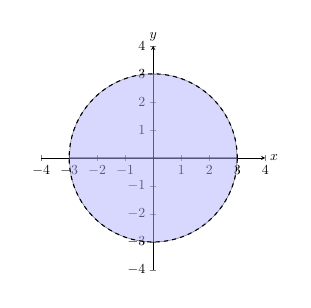
\begin{tikzpicture}[scale =0.5]
	      		\begin{axis}[
	      				xlabel=$x$,
	      				ylabel=$y$,
	      				xmin=-4,
	      				xmax=4,
	      				ymin=-4,
	      				ymax=4,
	      				axis equal image,
	      				axis lines=middle,
	      				xtick distance=1,
	      				ytick distance=1,
	      				xlabel style={at={(ticklabel* cs:1)}, anchor=west},
	      				ylabel style={at={(ticklabel* cs:1)}, anchor=south},
	      			]
	      				      			
	      			% Draw the shaded region for 9 > x^2 + y^2
	      			\addplot[fill=blue!30, domain=-3:3,opacity=0.5, samples=100, smooth] {sqrt(9 - x^2)} \closedcycle;
	      			\addplot[fill=blue!30, domain=-3:3,opacity=0.5, samples=100, smooth] {-sqrt(9 - x^2)} \closedcycle;
	      				      			
	      			% Draw the circle boundary (dashed)
	      			\draw[thick, dashed] (0,0) circle (3);
	      				      			
	      		\end{axis}
	      	\end{tikzpicture}
	      	\caption{Graph of the domain of $f(x,y)$}
	      \end{figure}
	      	      
	\item $g(x,y,z) =\sqrt{x^2+\frac{y^2}{9}+z^2-1} = \frac{1}{3}\sqrt{9x^2+y^2+9z^2-9}$
	      \begin{enumerate}
	      	\item \textbf{Domain: }$\{(x,y)\in \mathrm{R}^3: 9x^2+y^2+9z^2 \geq 9\}$
	      	\item \textbf{Range: } $g(x,y,z)\in(0,\infty)$
	      \end{enumerate}
	      \begin{figure}[h]
	      	\centering
	      	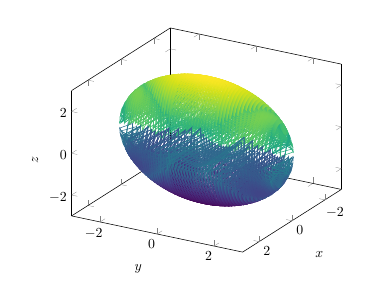
\begin{tikzpicture}[scale=0.5]
	      		\begin{axis}[
	      				xlabel=$x$,
	      				ylabel=$y$,
	      				zlabel=$z$,
	      				xmin=-3,
	      				xmax=3,
	      				ymin=-3,
	      				ymax=3,
	      				zmin=-3,
	      				zmax=3,
	      				view={120}{30},
	      				colormap/viridis,
	      			]
	      				      			
	      			% Plot the surface defined by 9 = 9x^2 + y^2 + 9z^2
	      			\addplot3[
	      				mesh,
	      				domain=-1:1,
	      				domain y=-3:3,
	      				samples=60,
	      				samples y=60,  % Increase the number of samples for a smoother plot
	      			] {sqrt(9 - 9*x^2 - y^2)};
	      				      			
	      			\addplot3[
	      				mesh,
	      				domain=-1:1,
	      				domain y=-3:3,
	      				samples=60,
	      				samples y=60,  % Increase the number of samples for a smoother plot
	      			] {-sqrt(9 - 9*x^2 - y^2)};
	      				      			
	      		\end{axis}
	      	\end{tikzpicture}
	      	\caption{Graph of the domain of $g(x,y,z)$}
	      \end{figure}
\end{enumerate}


\newpage
\subsection{}
Consider $z=f(x,y)=\frac{y^2}{25}-\frac{x^2}{16}$.
\subsubsection{}
Sketch a well-labelled contour map showing level curves $z = -1, 0, 1$.
	      \begin{figure}[h]
	      	\centering
	      	\begin{tikzpicture}
	      		\begin{axis}[
	      				xlabel=$x$,
	      				ylabel=$y$,
	      				title={$z = \frac{y^2}{25} - \frac{x^2}{16}$},
	      				axis equal,
	      				colormap/viridis,
	      				colorbar,
	      				view={0}{90}
	      			]
	      			                    
	      			\addplot3[
	      				contour gnuplot={
	      					number=12,
	      					labels=false,
	      				},
	      				samples=100,
	      				domain=-5:5,
	      				y domain=-5:5,
	      			] {y^2/25 - x^2/16};
	      			                    
	      		\end{axis}
	      	\end{tikzpicture}
	      	\caption{Contour Map}
	      \end{figure}
\subsubsection{}
Now, graph the traces in the $xz-$plane and the $yz-$plane. Note that the level curve $z = 0$ is the trace in the $xy-$plane.
	      	       
	      \begin{figure}[h]
	      	\centering
	      	\begin{subfigure}{0.3\textwidth}
	      		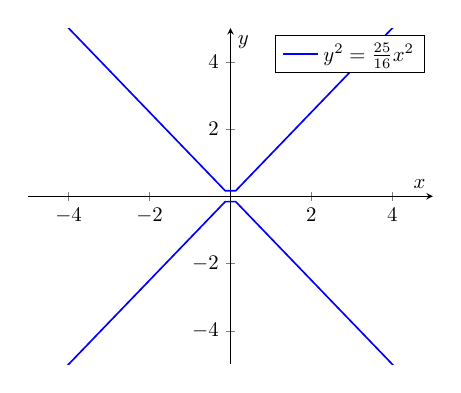
\begin{tikzpicture}[scale=0.75]
	      			\begin{axis}[
	      					xlabel=$x$,
	      					ylabel=$y$,
	      					axis lines=middle,
	      					xmin=-5, xmax=5,
	      					ymin=-5, ymax=5,
	      					samples=40, % Increase for smoother curve
	      					domain=-5:5,
	      				]
	      				\addplot+[color=blue,mark=none,thick,restrict y to domain=-10:10] {sqrt((25/16)*x^2)};
	      				\addplot+[color=blue,mark=none,thick,restrict y to domain=-10:10] {-sqrt((25/16)*x^2)};
	      				\addlegendentry{$y^2=\frac{25}{16}x^2$}
	      			\end{axis}
	      		\end{tikzpicture}
	      		\caption{$xy-$trace}
	      	\end{subfigure}
	      	\begin{subfigure}{0.3\textwidth}
	      		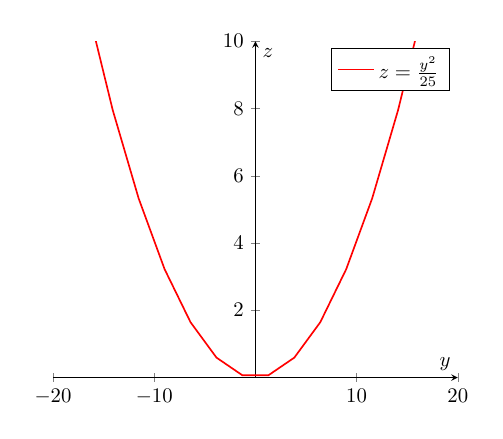
\begin{tikzpicture}[scale=0.75]
	      			\begin{axis}[
	      					xlabel=$y$,
	      					ylabel=$z$,
	      					axis lines=middle,
	      					xmin=-20, xmax=20,
	      					ymin=0, ymax=10,
	      					samples=40, % Increase for smoother curve
	      					domain=-50:50,
	      				]
	      				\addplot+[color=red,mark=none,thick,restrict y to domain=-50:50] {(x^2)/25};
	      				\addlegendentry{$z=\frac{y^2}{25}$}
	      			\end{axis}
	      		\end{tikzpicture}
	      		\caption{$yz-$trace}
	      	\end{subfigure}
	      	\begin{subfigure}{0.3\textwidth}
	      		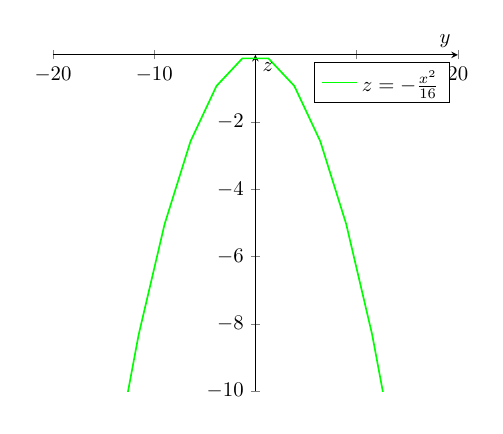
\begin{tikzpicture}[scale=0.75]
	      			\begin{axis}[
	      					xlabel=$y$,
	      					ylabel=$z$,
	      					axis lines=middle,
	      					xmin=-20, xmax=20,
	      					ymin=-10, ymax=0,
	      					samples=40, % Increase for smoother curve
	      					domain=-50:50,
	      				]
	      				\addplot+[color=green,mark=none,thick,restrict y to domain=-50:50] {-(x^2)/16};
	      				\addlegendentry{$z=-\frac{x^2}{16}$}
	      			\end{axis}
	      		\end{tikzpicture}
	      		\caption{$yz-$trace}
	      	\end{subfigure}
	      \end{figure}
	      \newpage
\subsubsection{}
Graph the three-dimensional surface.  
 \begin{figure}[h]
	      	\centering
	      	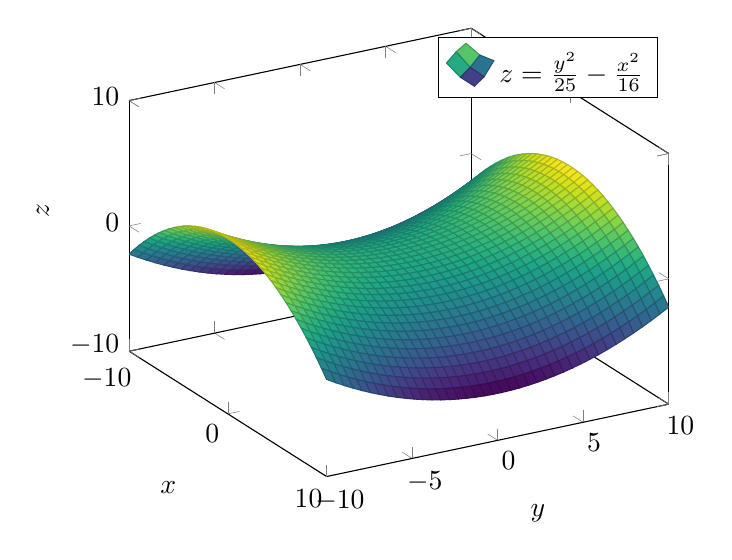
\begin{tikzpicture}
	      		\begin{axis}[
	      				xlabel=$x$,
	      				ylabel=$y$,
	      				zlabel=$z$,
	      				domain=-10:10,
	      				y domain=-10:10,
	      				zmin=-10,
	      				zmax=10,
	      				samples=40,
	      				colormap/viridis,
	      				view={60}{30},
	      			]
	      			\addplot3[surf] {y^2/25 - x^2/16};
	      			\addlegendentry{\(z=\frac{y^2}{25}-\frac{x^2}{16}\)}
	      		\end{axis}
	      	\end{tikzpicture}
	      \end{figure}


\end{document}
